\section{Cartograms with Dynamic Features}

{
\begin{figure}[tb!]
    \centering
    \includegraphics[width=\columnwidth]{example-image-a}
    \caption{An screenshot of \software. Figure TBA.}
    \label{fig:overview}
\end{figure}
}

{
\begin{figure}[tb!]
    \centering
    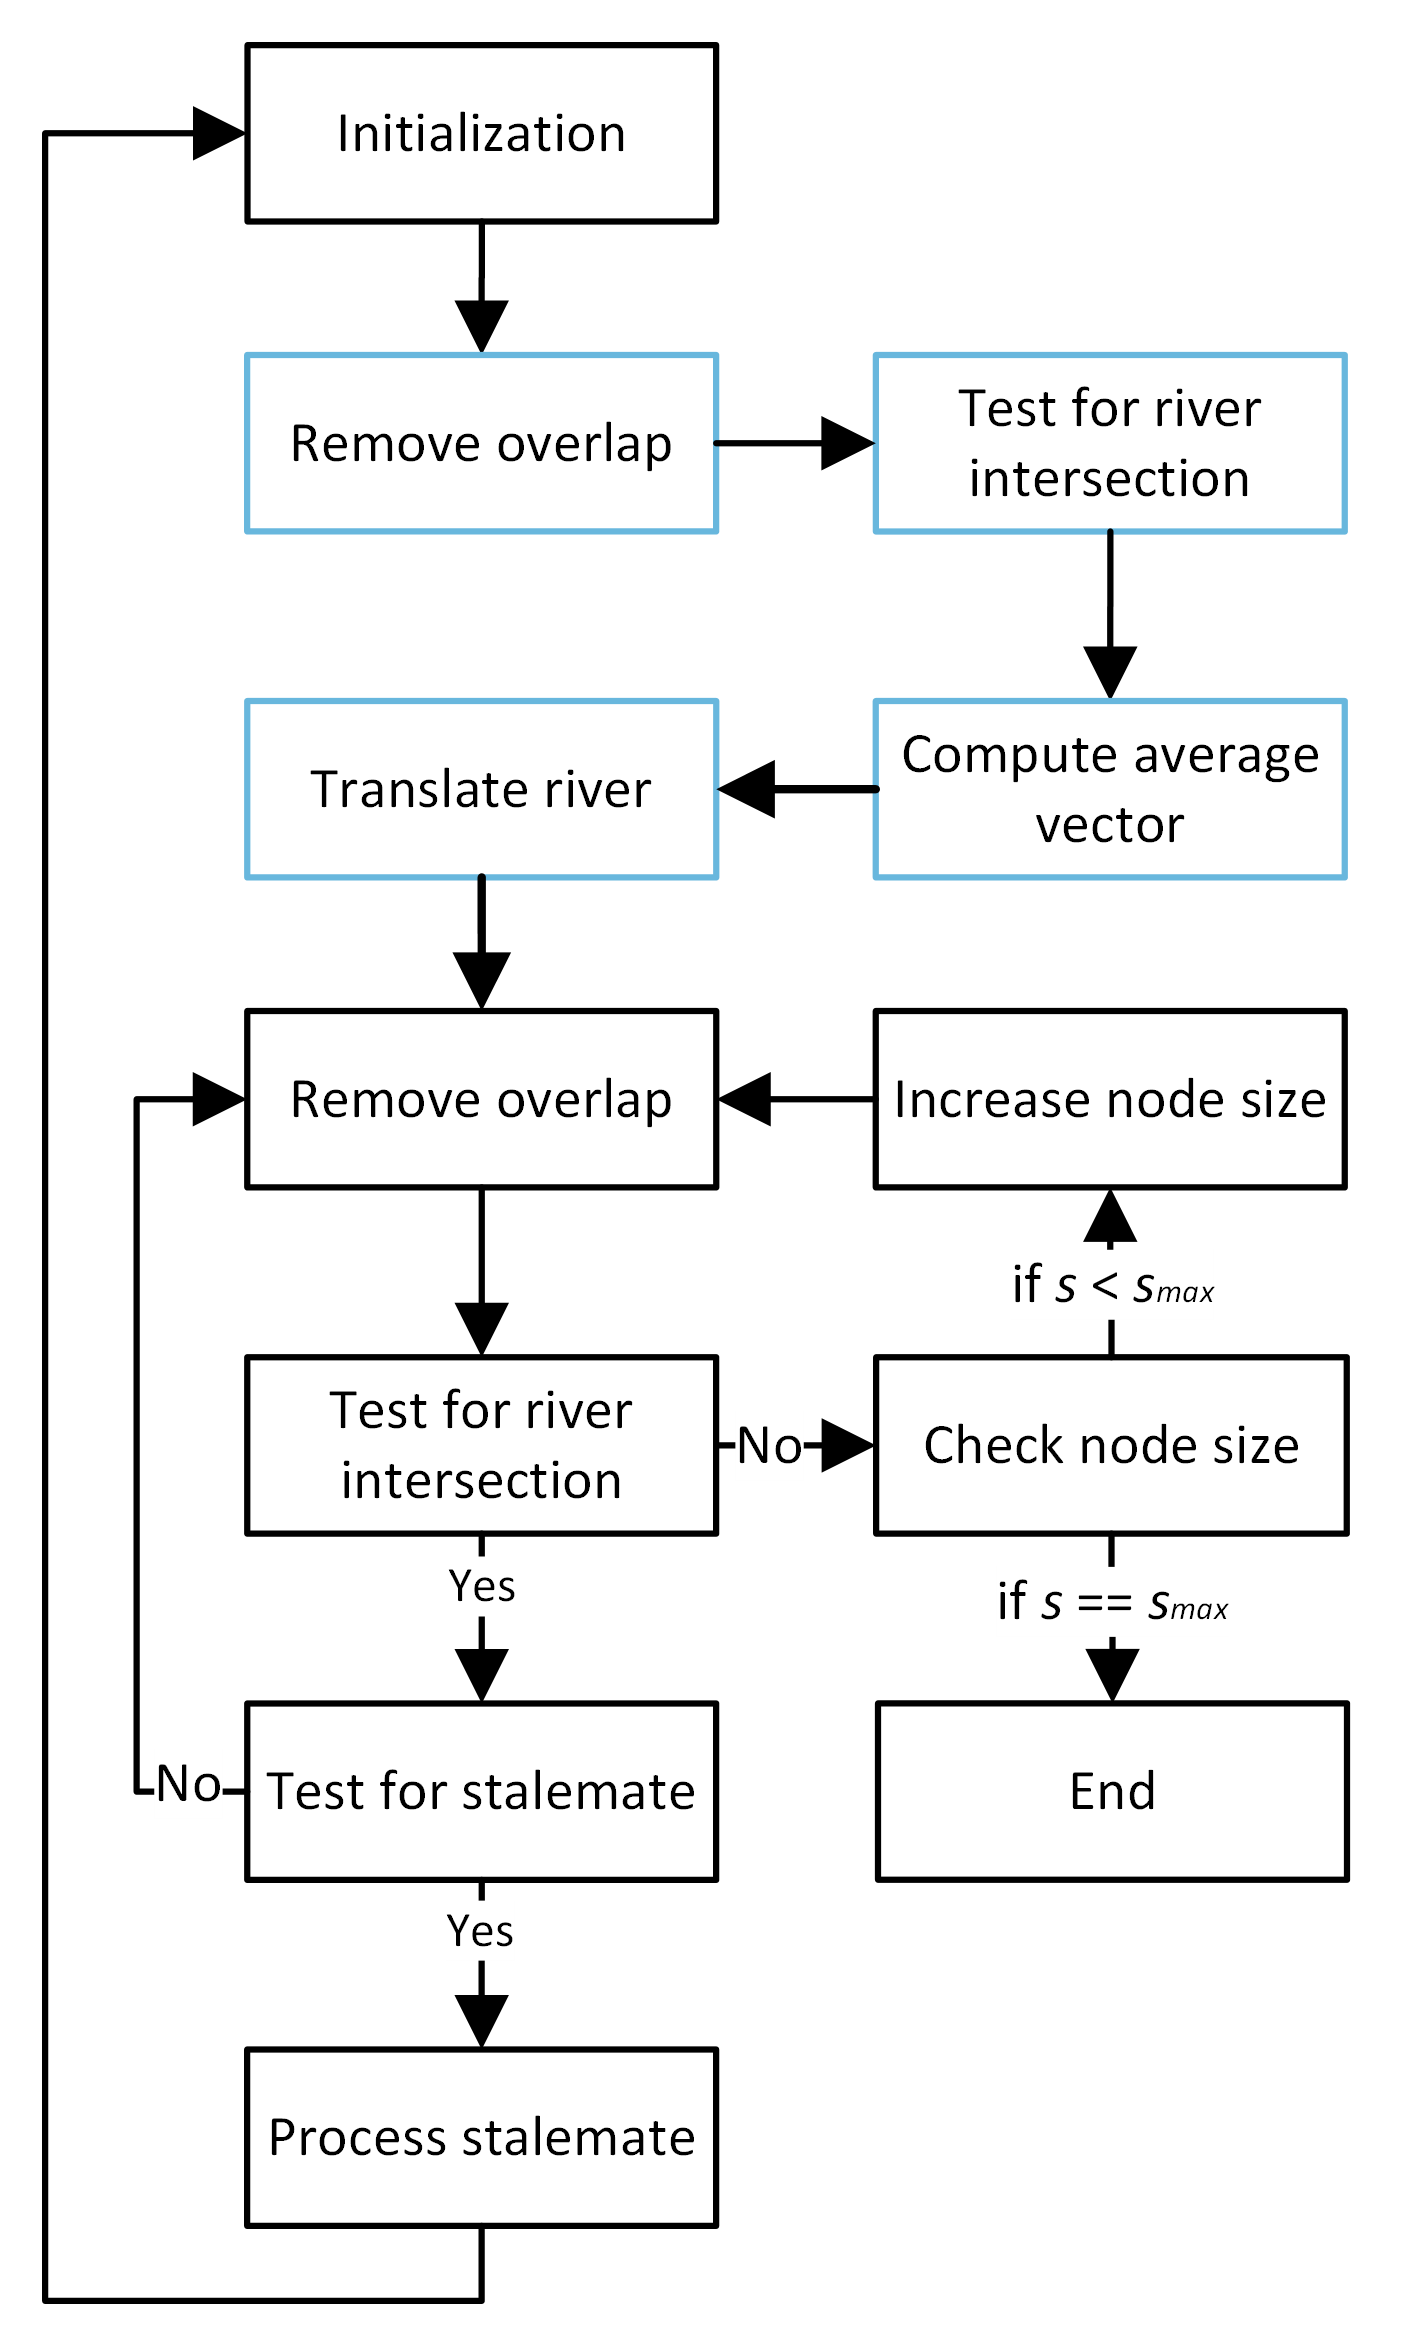
\includegraphics[width=\columnwidth]{figure/flowchart.png}
    \caption{A flowchart showing the abstraction of our layout algorithm.}
    \label{fig:flowchart}
\end{figure}
}

\algoref{alg:UpdateNodePosition} and \figref{fig:flowchart} provide an overview of our algorithm. \textbf{Initialization:} We first load and render the CCG geospatial boundaries. For each CCG we compute the centroid and represent it using a small unit size square node with $ \nodeSize $ as the initial size. \textbf{Node layout:} The basic algorithm is as follows: we first apply the Fast Node Overlap Removal (VPSC) algorithm \cite{dwyer2006fast} to remove overlaps. We chose VPSC over other node overlap removal algorithms since VPSC is able to provide spread minimization and node movement minimization while maintaining a good level of global shape preservation \cite{chen2020Node}. During overlap removal, we compute node trajectories (See \algoref{alg:check river intersection}) and translate nodes to their new position. Nodes that cross a river are translated back to their previous position. This procedure ends when 1) no node overlap is present; 2) no nodes cross a river. We then increase $ \nodeSize $ by one pixel and repeat the algorithm until the max node size $ \nodeSizeMax $ is reached. \new{The size growing process provides a stability in the layout and minimizes geographical errors.}

% \begin{noindent}

\begin{algorithm}[tb!]
    \caption{Procedure to update node positions by removing overlap and prevent nodes from crossing rivers.}\label{alg:UpdateNodePosition}
    \textbf{Global variables:} \\
    $ \nodeList \gets $ a list of nodes representing CCGs \\
    $ \nodeSize \gets $ the current size of all nodes \\
    $ \nodeSizeMax \gets $ the maximum size of a node \\
    $ \stalemateMax \gets $ the maximum number of iterations indicating a stalemate \\

    \textbf{Local variables:} \\
    $ \nodeListVPSC \gets $ a list of nodes representing CCGs after VPSC \\
    $ \nodeListCross \gets True $ if any node in the list crossed a river \\
    $ \nodeCross \gets True $ if the node crossed a river \\
    $ \nodeListEach \gets $ a node in $ \nodeList $ \\
    $ \nodeListEachPrevious \gets $ the previous position of $ \nodeListEach $\\
    $ \nodeListVPSCEach \gets $ a node in $ \nodeListVPSC $, which is the position of $ \nodeListEach $ after VPSC \\

    \begin{algorithmic}[1]
        \Procedure{UpdateNodePosition}{}
        \While{$ \nodeSize < \nodeSizeMax $}

            \While{$ \nodeListCross = True $}

                \State $ \nodeListCross \gets False $
                \State $ \nodeListVPSC \gets $ RemoveOverlap ($ \nodeList $)

                \ForEach {$ \nodeListVPSCEach \in \nodeListVPSC $}

                    \If {$ \nodeListEach(x,y) \neq \nodeListVPSCEach(x,y) $}

                        \State $ \nodeCross \gets $ \Call{TestRiverIntersection}{$ \nodeListVPSCEachLine $}
                        \State $ \nodeListEach(x,y) \gets \nodeListVPSCEach(x,y) $

                        \If{$ \nodeCross = True $}

                            \State $ \nodeListCross \gets True $
                            \State $ \nodeListEachStalemate \gets \nodeListEachStalemate + 1 $

                            \If{$ \nodeListEachStalemate < \stalemateMax $}

                                \State $ \nodeListEach(x,y) \gets \nodeListEachPrevious(x,y) $

                            \Else

                                \State \Call{ProcessStalemate}{$ \nodeListEach, \nodeListVPSCEach $}
                                \State $ \nodeListEachStalemate \gets 0 $ \Comment{Reset counter}

                            \EndIf
                            
                        \EndIf

                    \EndIf

                \EndFor

            \EndWhile

            \State $ \nodeSize \gets \nodeSize ++$

        \EndWhile

        \EndProcedure
    \end{algorithmic}
\end{algorithm}


% \begin{algorithm}[tb!]
%     \caption{Procedure to update the position of a single node $ \node $.}\label{alg:move position}

%     \textbf{Input:} \\
%     $ \node \gets $ the node \\
%     $ \nodeVPSC \gets $ the node after running VPSC \\

%     \textbf{Output:} \\
%     Returns $ True $ if the node's position is updated. \\

%     \begin{algorithmic}[1]
%         \Procedure{TranslateNode}{$ \node, \nodeVPSC $}
%         \If{$ \node(x,y) = \nodeVPSC(x,y) $}
%             \item[] \Comment{Node position remains unchanged}
%             \State \Return{$ False $}
%         \EndIf

%         \State $ \node(x,y) \gets \nodeVPSC(x,y) $

%         \State \Return{$ True $}
%         \EndProcedure
%     \end{algorithmic}
% \end{algorithm}

%\end{noindent}

\subsection{River Intersection Testing}

We use rivers as topological boundaries and prevent nodes from crossing them. The resolution of rivers can be adjusted by the user, as shown in \figref{fig:river resolution}, the number of edges is reduced from 10,170 to 65. Enabling river simplification reduces the number of edge intersection tests that need to be performed. When a node's position changes, we test if the node's trajectory intersects any segment of a river. See \algoref{alg:check river intersection}. A bounding box intersection test between the edge defined by node translation and river edges can be performed to reduce the number of edge intersection detections required.


{
\begin{figure}[tb!]
    \centering
    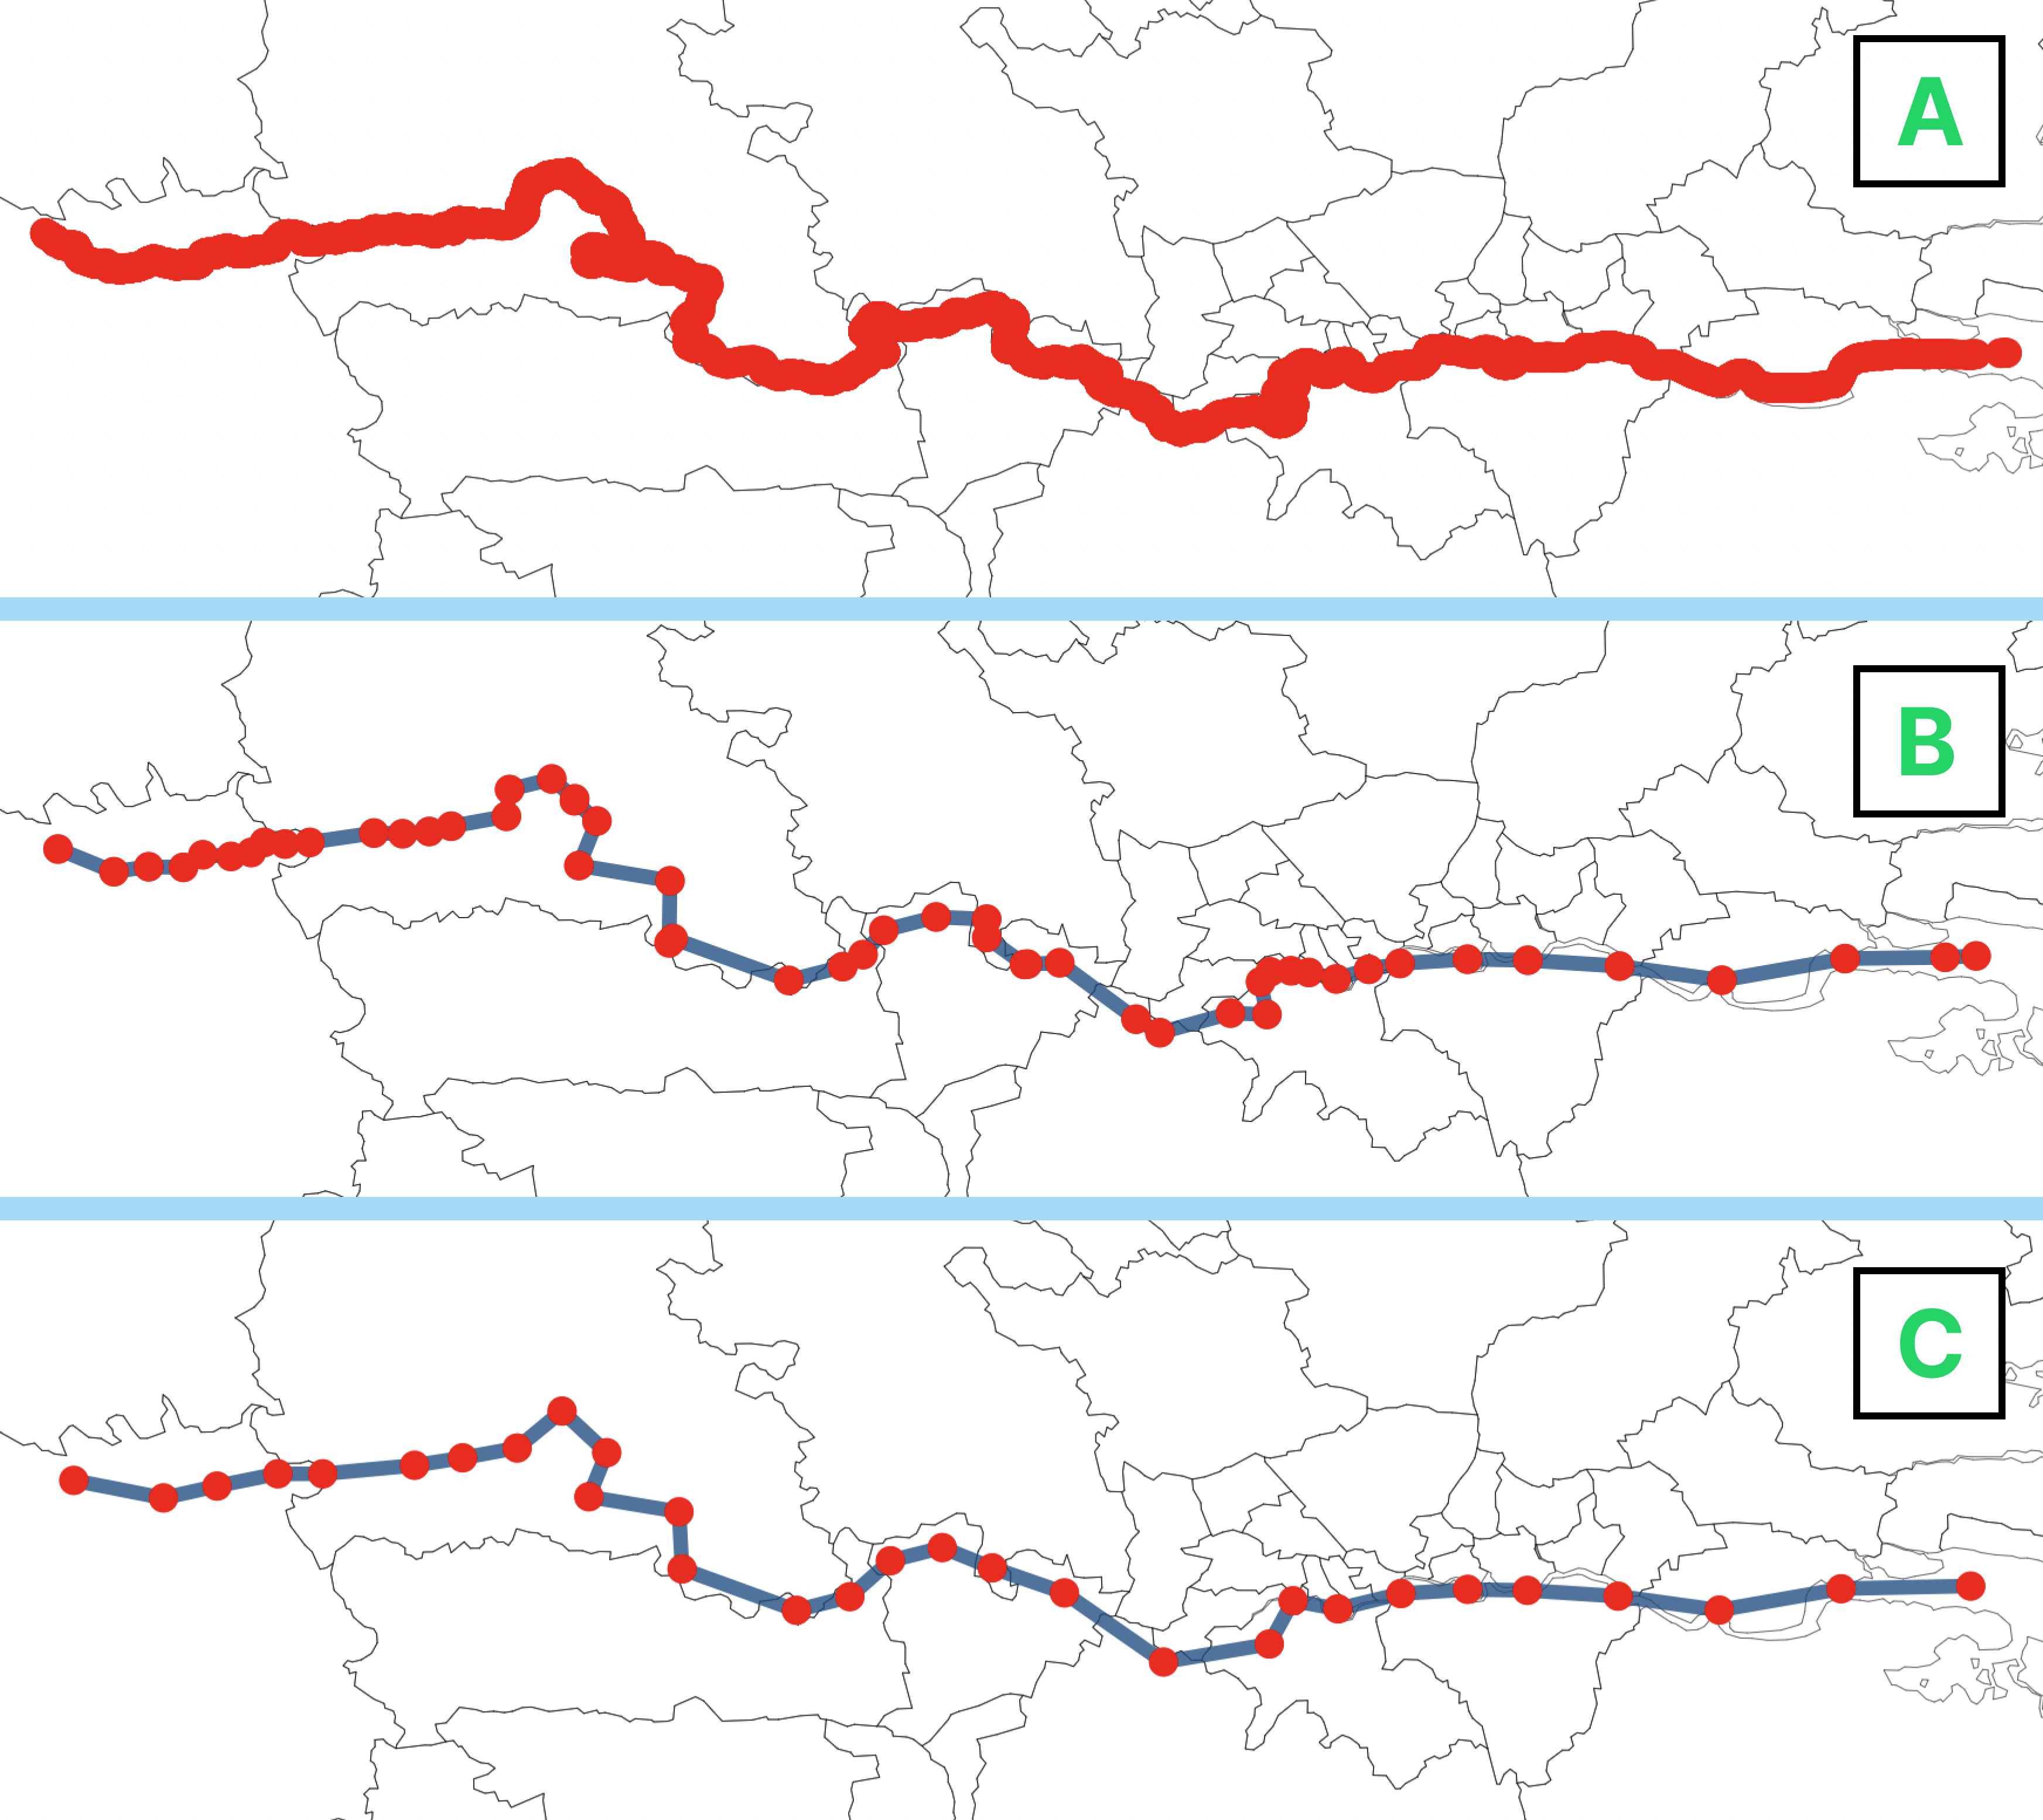
\includegraphics[width=\columnwidth]{figure/river_resolution.png}
    \caption{The resolution of rivers can be dynamically adjusted by the user. The top figure shows River Thames at its original resolution with 10,170 edges. The bottom figure shows the river at a  reduced resolution of 65 edges. The reduced resolution preserves the majority of River Thames' original shape and improves the performance of our river intersection tests.}
    \label{fig:river resolution}
\end{figure}
}

% \begin{noindent}
\begin{algorithm}[tb!]
    \caption{Procedure to test if a node's translation path, $ \nodeLineNV $ intersects a river.}\label{alg:check river intersection}
    \textbf{Input:} \\
    $ \nodeLineNV \gets $ the node's translation path \\

    \textbf{Output:} \\
    Returns $ True $ if the node crosses a river. \\

    \textbf{Global variables:} \\
    $ \riverEdgeList \gets $ a list of river edges \\

    \textbf{Local variables:} \\
    $ \riverEdgeListEachLine \gets $ a river edge in $ \riverEdgeList $ \\ 
    $ \nodeBoundingBox, \riverEdgeBoundingBoxEach \gets $ the bounding boxes for $ \nodeLineNV $ and $ \riverEdgeListEachLine $ \\
    % $ \boundingBoxInt \gets $ boolean indicating $ \nodeBoundingBox $ intersects $ \riverEdgeBoundingBoxEach $ \\
    % $ \nodeEdge \gets $ the edge for $ \node $\\
    % $ \edgeBoxInt \gets $ boolean indicating $ \nodeEdge $ intersects $ \riverEdgeListEach $ \\

    \begin{algorithmic}[1]
        \Procedure{TestRiverIntersection}{$ \nodeLineNV $}
        
        \ForEach{$ \riverEdgeListEachLine \in \riverEdgeList $}
            \State $ \nodeBoundingBox \gets $ GetBoundingBox ($ \nodeLineNV $)
            \State $ \riverEdgeBoundingBoxEach \gets $ GetBoundingBox ($ \riverEdgeListEachLine $)
            % \State $ \boundingBoxInt \gets $ TestIntersection ($ \nodeBoundingBox, \riverEdgeBoundingBoxEach $)
            % \If{$ \boundingBoxInt = True $}

            \If{$ \nodeBoundingBox ~intersect~ \riverEdgeBoundingBoxEach = True $}
                \State \Return{$ \nodeLineNV ~intersect~ \riverEdgeListEachLine $}
                \EndIf
        \EndFor
        
        \State \Return{$ False $}
        \EndProcedure
    \end{algorithmic}
\end{algorithm}
%\end{noindent}

\subsection{Detecting Stalemates}

As the VPSC always tries to produce an optimal node layout where node distribution and translation are minimized, a node's translation path might be repeatedly intersecting a river due to congestion, creating a stalemate situation, as shown in \figref{fig:stalemate}. If a node is translated between two positions for $ \stalemateMax $ iterations, a corridor is derived to break up the congestion. A corridor, $ c $, is a rectangle with a width of $ \CorridorWidth $ and a length of $ \CorridorLength $, formed by deriving two edges $ \EdgeParallelA $ and $ \EdgeParallelB $ such that $ \EdgeParallelA \parallel \EdgeParallelA \parallel \nodeLineNpP $ (See \figref{fig:corridor}C and D). All enclosed nodes are then translated by $ \nodeVectorPC $ to alleviate the congestion (See \figref{fig:corridor}D).

{
\begin{figure}[tb!]
    \centering
    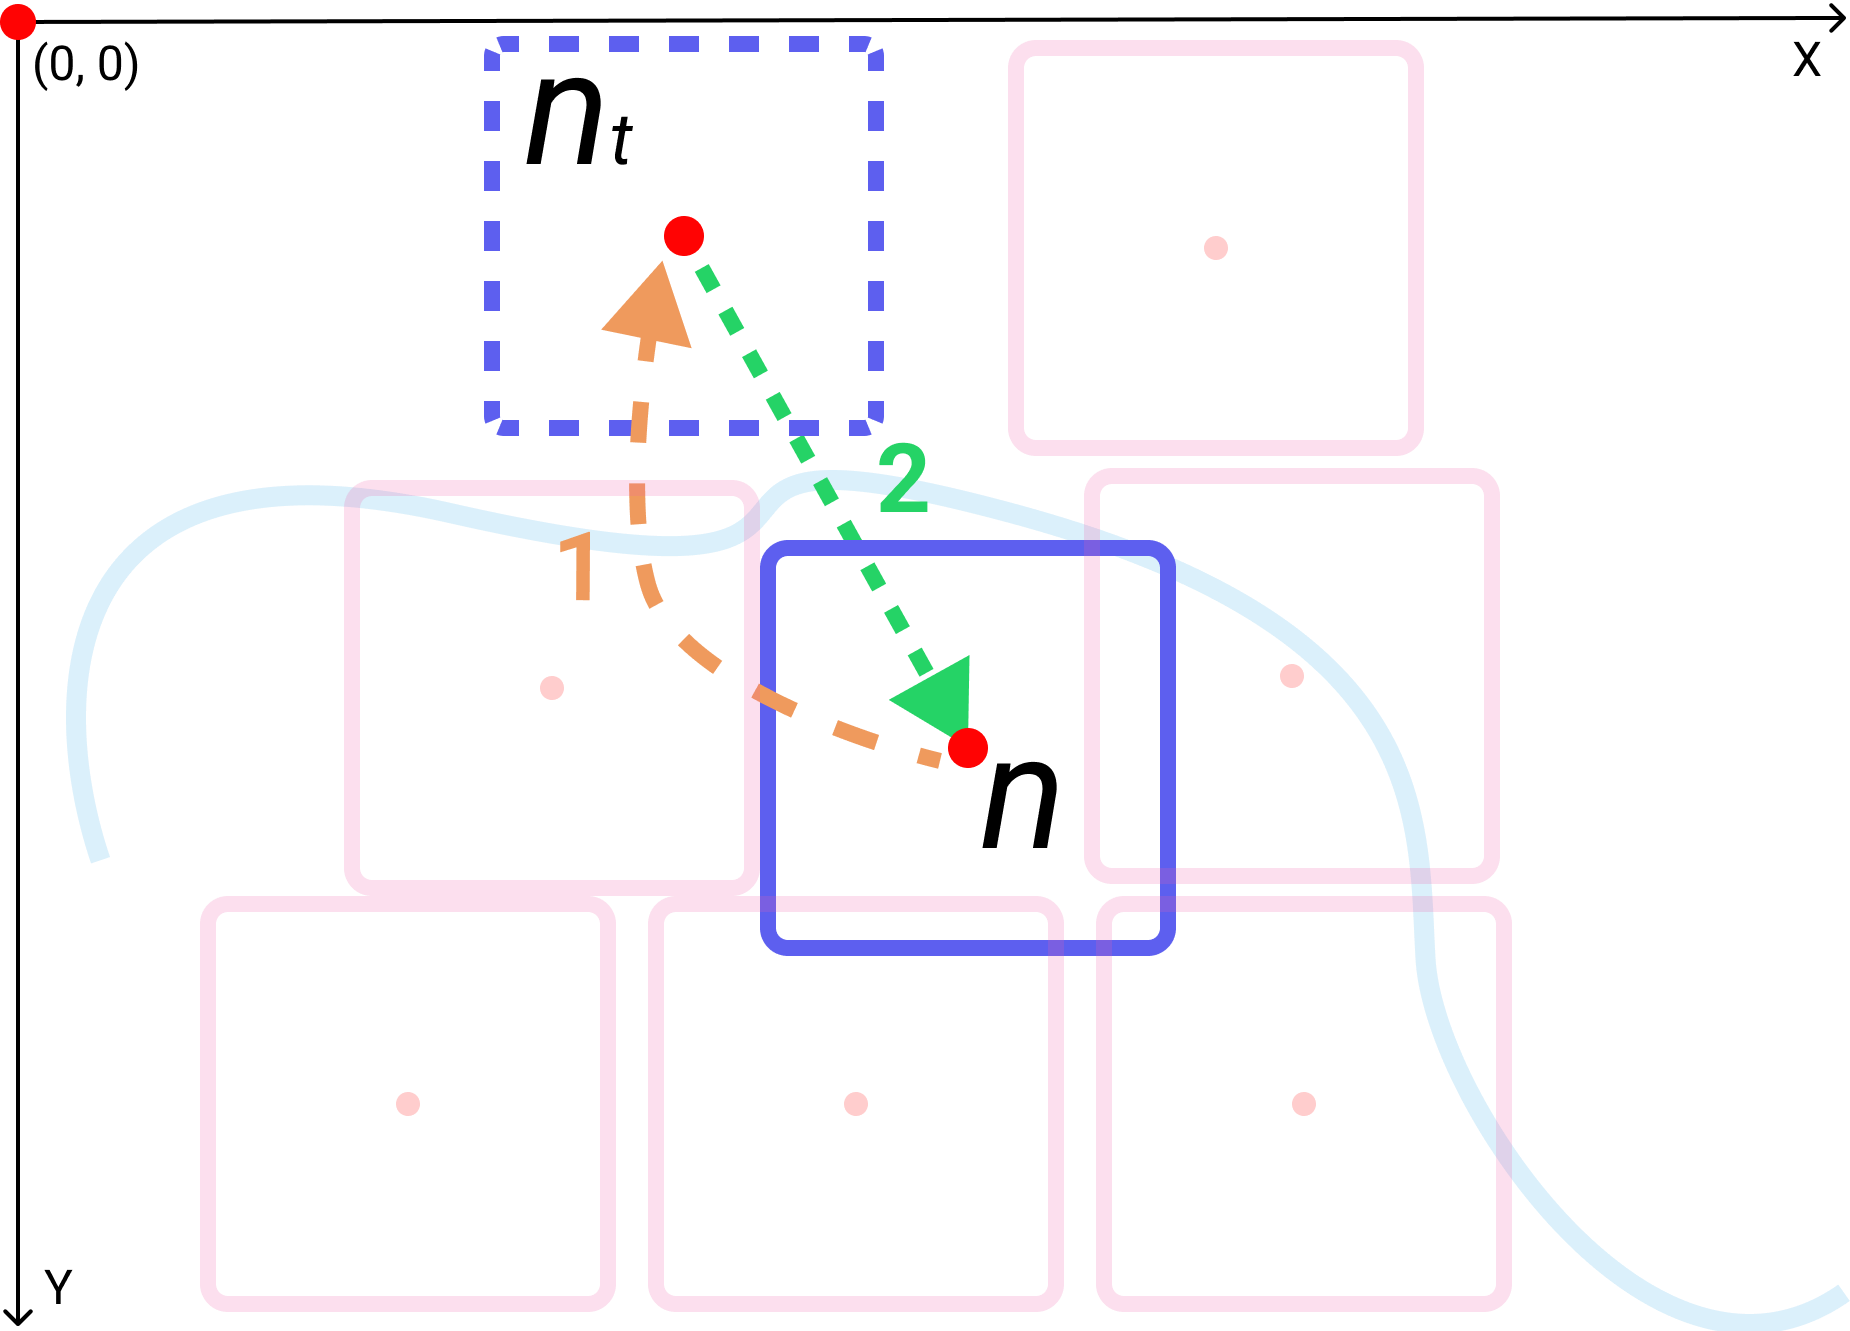
\includegraphics[width=\columnwidth]{figure/stalemate.png}
    \caption{A stalemate situation is when a node's translation path $ \nodeVectorCP $ intersects a river for $ \stalemateMax $ times. A stalemate often occurs when the area is congested and the node is unable to move to a position that is not intersecting a river.}
    \label{fig:stalemate}
\end{figure}
}

{
\begin{figure}[tb!]
    \centering
    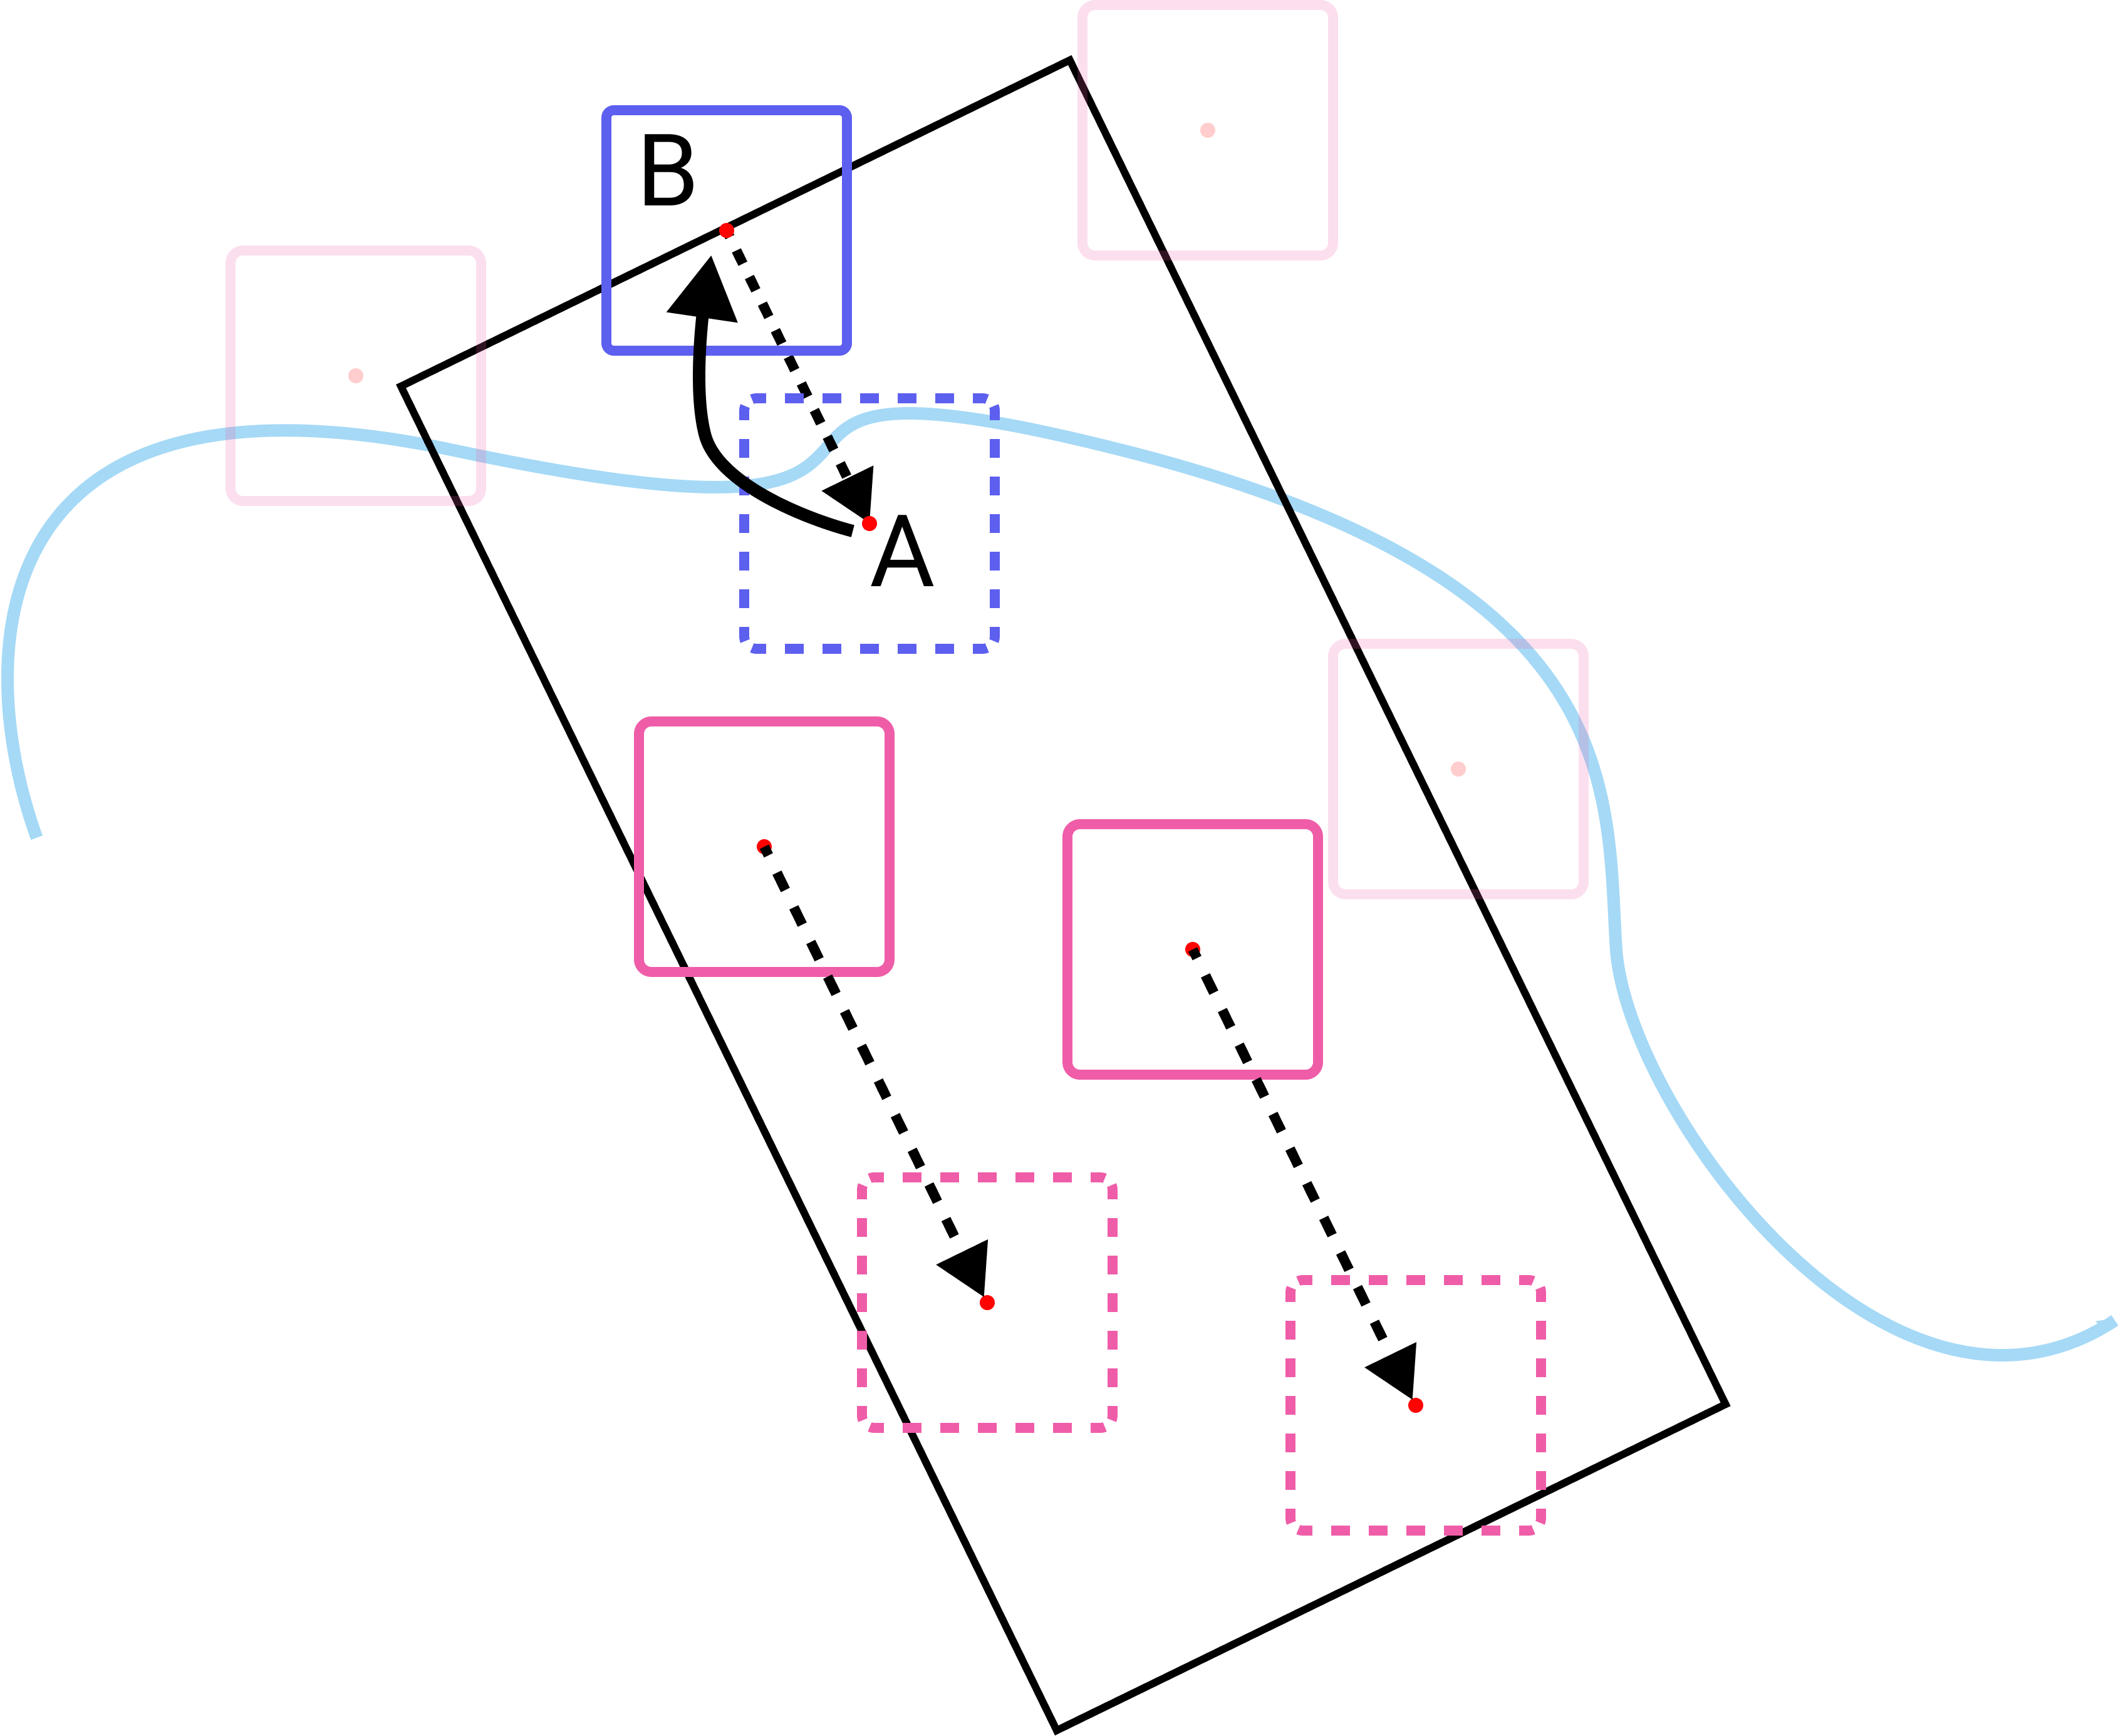
\includegraphics[width=\columnwidth]{figure/corridor.png}
    \caption{A stalemate occurs when a node's translation path $ \nodeVectorCP $ intersects a river for $ \stalemateMax $ times, as shown in A. To address the issue, we derive a corridor (orange rectangle in D) based on $ \node $ and $ \nodePrevious $. All nodes within the corridor are translated based on $ \nodeVectorPC $, such that $ \nodeVectorPC = \nodeVectorNNn = \nodeVectorNinNinn $. In order to show a clear illustration, we place nodes sparsely in this figure.}
    \label{fig:corridor}
\end{figure}
}

% \begin{noindent}

\begin{algorithm}[tb!]
    \caption{Procedure to derive a corridor to translate enclosed nodes. We use an SVG canvas, where the point of origin (0,0) is located at the top left corner, with the x-axis extending to the right and the y-axis extending downwards (See \figref{fig:stalemate}).}\label{alg:derive corridor}

    \textbf{Input:} \\
    $ \node \gets $ the node used to derive the corridor \\

    \textbf{Global variables:} \\
    $ \CorridorLength \gets $ the length of a corridor \\
    $ \CorridorWidth \gets $ the width of a corridor \\

    \textbf{Local variables:} \\
    $ \Corridor \gets $ the corridor \\
    $ \nodePrevious \gets $ the previous position of $ \node $ \\
    $ \PointP \gets $ the point extending $ \nodeVectorPC $ such that $ \nodeLineWidthNpP = \CorridorLength $\\
    $ \EdgeParallelA, \EdgeParallelB \gets $ the edges parallel to $ \nodeLineNpP $ \\
    $ corridor \gets $ a rectangle formed by $ \EdgeParallelA $ and $ \EdgeParallelB $ \\

    \begin{algorithmic}[1]
        \Procedure{ProcessStalemate}{$ \node $}
            \State $ \node(x,y) \gets \nodePrevious(x,y) $

            \State $ \PointP \gets $ \Call{DerivePoint}{$ \nodeVectorPC $, $ \CorridorLength $}

            \State $ \EdgeParallelA \gets $ \Call{DeriveParallelEdge}{$ \nodeVectorNpP $, $ \frac{\CorridorWidth}{2} $}

            \State $ \EdgeParallelB \gets $ \Call{DeriveParallelEdge}{$ \nodeVectorNpP $, $ -\frac{\CorridorWidth}{2} $}

            \State $ \Corridor \gets
                \begin{bmatrix}
                    \EdgeParallelA.start &
                    \EdgeParallelA.end \\

                    \EdgeParallelB.start &
                    \EdgeParallelB.end \\
                \end{bmatrix} $

            \ForEach{$ \nodeInCorridorEach $ inside $ \Corridor $}

                \State $ \Vector{\nodeInCorridorEach ~\nodeInCorridorEachT} = \nodeVectorPC $

                \State $ \nodeInCorridorEach(x,y) \gets \nodeInCorridorEachT(x,y) $

            \EndFor
        \EndProcedure
    \end{algorithmic}
\end{algorithm}

%\end{noindent}
